\chapter{Modelos Basados en Energía y Aprendizaje de Compatibilidades}
\label{cap:ebm_compatibilidades}

\input{cap2_introEBM}
\section{Introducción a los Energy-Based Models y el Paisaje de Energía}
\label{sec:intro_ebm}

Los Modelos Basados en Energía (EBM) ofrecen un marco matemático flexible para el diseño de sistemas de inteligencia artificial \cite{lecun2006tutorial}. En el contexto de este trabajo, constituyen la base formal de las \textbf{Joint Embedding Architectures (JEA)}. A diferencia de los modelos probabilísticos, que requieren una  normalización estricta, los EBM evalúa la compatibilidad entre variables asignándoles un escalar no normalizado denominado "energía". Intuitivamente, una energía baja indica que la combinación de variables es altamente plausible o compatible, mientras que una energía alta denota incompatibilidad. Esta métrica se puede visualizar como un "paisaje de energía" donde los valles (mínimos locales) representan las configuraciones de interés, y las cimas (picos de energía) representan configuraciones "implausibles" o ruido. Si el modelo fracasa y mapea cualquier combinación a la misma energía (por ejemplo, a cero), el paisaje de energía se aplana completamente. Este  fenómeno destructivo se le conoce como \textbf{colapso de representación}.

\subsection{La Función de Energía y su Independencia Probabilística}
\label{sec:energy_function}

En tareas de predicción y aprendizaje de representaciones (como las JEA), el modelo opera sobre el espacio conjunto de configuraciones, definido como el espacio producto $\mathcal{C} = \mathcal{X} \times \mathcal{Y}$, donde $x \in \mathcal{X}$ representa la variable observada o entrada del sistema (por ejemplo, el contexto de una imagen o fotograma) e $y \in \mathcal{Y}$ es la predicción o variable de destino a evaluar, La pieza central del modelo es la función de energía condicional:
\begin{equation}
E_\theta(x, y) \in \mathbb{R}
\end{equation}
siendo $\theta$ los parámetros entrenables del modelo (pesos de la red neuronal). El escalar $E_\theta(x, y)$ mide directamente la \textbf{discrepancia} entre $x$ e $y$. Esta energía se caracteriza por su total independencia de los axiomas de Kolmogorov:
\begin{itemize}
    \item \textbf{No negatividad:} A diferencia de las densidades de probabilidad, $E_\theta(x, y)$ puede tomar valores reales negativos.
    \item \textbf{Normalización:} No requiere que la integral sobre el espacio de predicción sume la unidad: $\int_{\mathcal{Y}} E_\theta(x, y') \, dy' \neq 1$.
\end{itemize}

Esta flexibilidad permite a las JEA centrarse exclusivamente en la superficie de energía, evitando calcular constantes de normalización complejas y canalizando la capacidad del modelo a la dinámica semántica de los datos en sus representaciones.

\subsection{Inferencia en Modelos Basados en Energía}
Realizar inferencia en un EBM consiste en buscar el estado \textbf{y} que minimiza la energía para una entrada observada $x$ dada. A diferencia del enfoque probabilístico que calcula expectativas o integrales sobre todo el espacio de salida, la inferencia no normalizada se reduce a un problema de optimización o búsqueda del mínimo global:
\begin{equation}
\label{eq:ebm_inferencia}
y^* = \arg\min_{y \in \mathcal{Y}} E_\theta(x, y)
\end{equation}

En la Figura~\ref{fig:ebm_inferencia_retriever}, se ilustra esta idea para el caso de clasificación de imágenes. Dada una entrada observada $x$ (la imagen de un perro), el modelo evalúa la energía $E_\theta(x, y)$ para cada una de las clases candidatas $y$. La respuesta inferida es la clase que produce el valor de energía mínimo (representado por la barra más corta).

\begin{figure}[H]
    \centering
    \begin{tikzpicture}[
        >=stealth,
        textfont/.style={font=\small\sffamily, align=center},
        labelsbox/.style={draw, align=left, inner sep=1.5ex, font=\small\sffamily, text depth=0pt}
    ]
        \node (img) {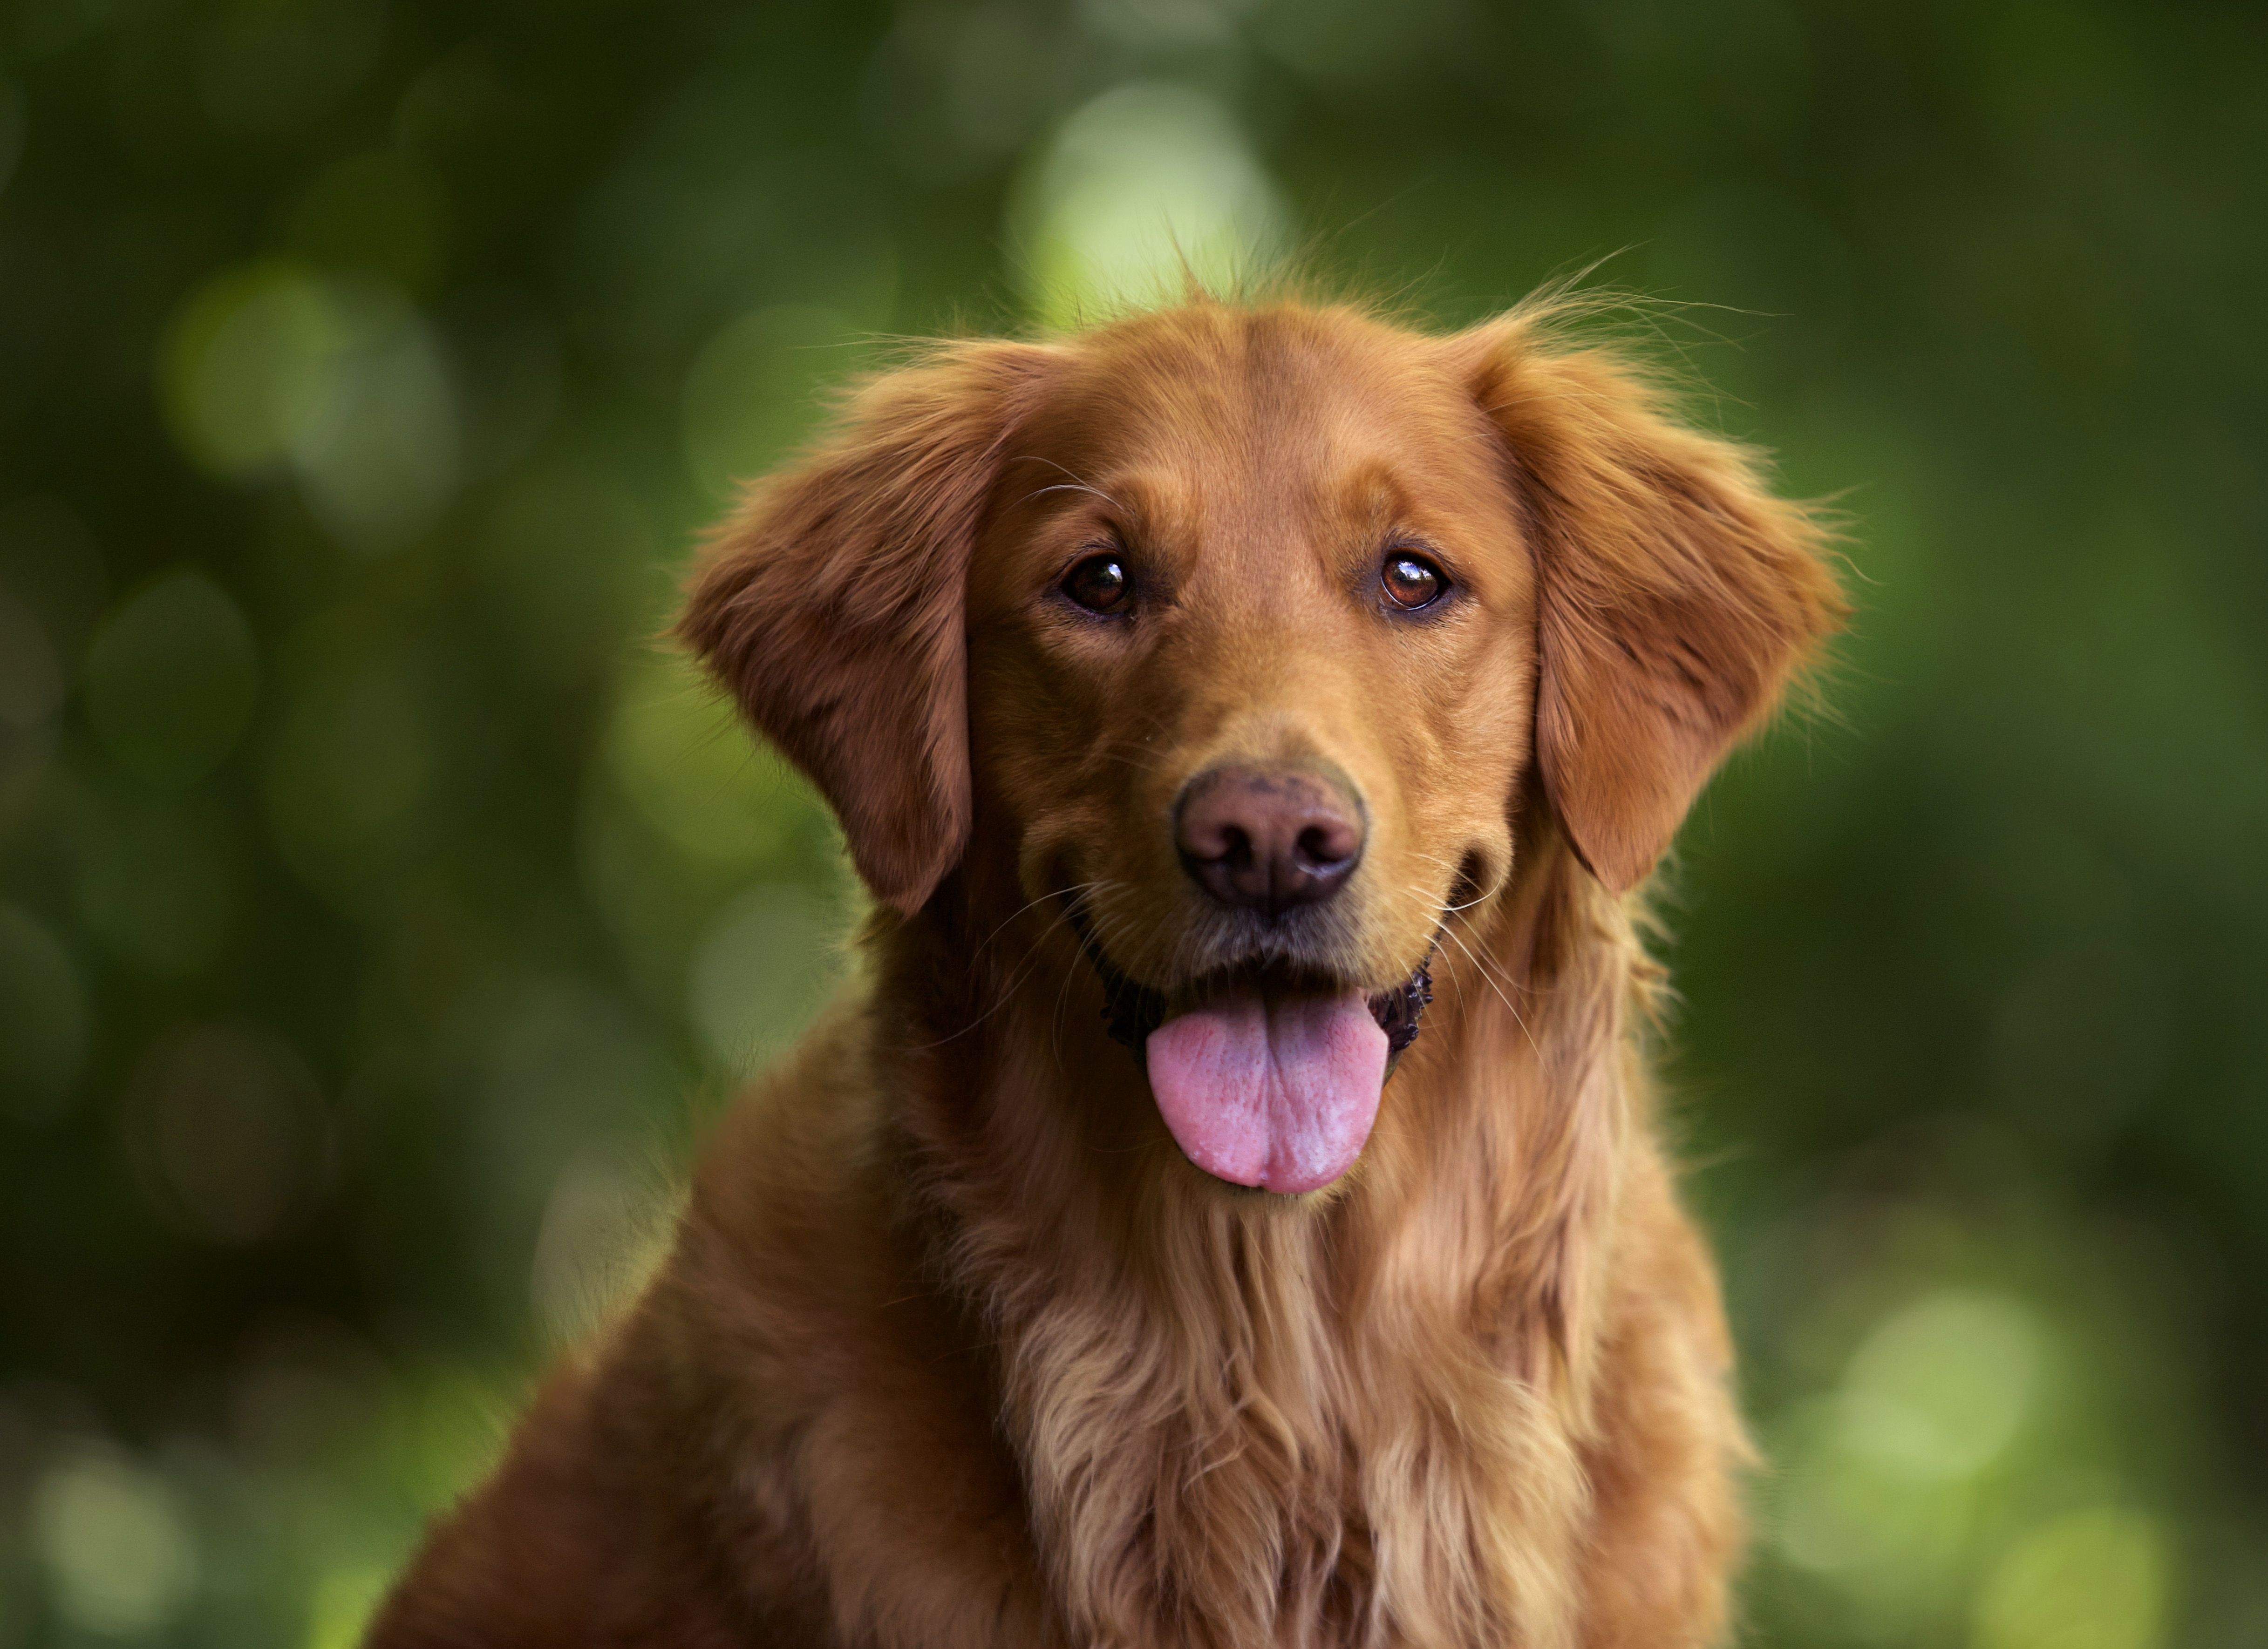
\includegraphics[width=3.5cm]{selective-focus-shot-adorable-golden-retriever-outdoors.jpg}};
        \node[above=0.2cm of img, textfont] (x_text) {$x$\\Variables observadas\\(input)};

        \node[right=2.5cm of img, labelsbox] (y_box) {
            Human \\ Animal \\ Airplane \\ Car \\ Truck
        };
        \node[above=0.2cm of y_box, textfont] (y_text) {$y$\\Variables a predecir\\(clase)};

        \node[draw, rounded corners, minimum width=8.5cm, minimum height=1.2cm,
              above=1.5cm of $(x_text.north)!0.5!(y_text.north)$,
              font=\normalsize\sffamily] (ef) {Función de Energía\quad $E_\theta(x, y)$};

        \draw[->, thick] (x_text) -- (x_text |- ef.south);
        \draw[->, thick] (y_text) -- (y_text |- ef.south);
        \draw[->, thick] (ef.north) -- ++(0, 1.2cm) coordinate (out_arrow);
        \node[right=0.1cm of out_arrow, yshift=-0.6cm, font=\small\sffamily] {};

        \begin{scope}[shift={($(ef.north)+(0, 1.3cm)$)}]
            \tikzset{bar/.style={draw, fill=gray!70, minimum height=0.2cm,
                     inner sep=0pt, anchor=west}}
            \node[left, font=\scriptsize\sffamily] at (0, 1.2) {Human};
            \node[bar, minimum width=1.5cm] at (0.1, 1.2) {};
            \node[left, font=\scriptsize\sffamily] at (0, 0.9) {Animal};
            \node[bar, minimum width=0.3cm] at (0.1, 0.9) {};
            \node[left, font=\scriptsize\sffamily] at (0, 0.6) {Airplane};
            \node[bar, minimum width=1.8cm] at (0.1, 0.6) {};
            \node[left, font=\scriptsize\sffamily] at (0, 0.3) {Car};
            \node[bar, minimum width=1.2cm] at (0.1, 0.3) {};
            \node[left, font=\scriptsize\sffamily] at (0, 0.0) {Truck};
            \node[bar, minimum width=0.9cm] at (0.1, 0.0) {};
            \draw[->, thick] (0.1, -0.2) -- (2.2, -0.2);
            \node[below, font=\scriptsize\sffamily] at (1.15, -0.2) {$E_\theta(x, y)$};
        \end{scope}
    \end{tikzpicture}
    \caption{Energía en el contexto de EBMs para una tarea de clasificación. Dada la entrada observada $x$ (imagen de un perro), el modelo evalúa la energía $E_\theta(x, y)$ para cada clase candidata $y$. La respuesta inferida es $y = \text{Animal}$, dado que tiene asociado el valor mínimo de energía de entre las posibles clases candidatas (barra más corta). Se observa, por tanto, que no requiere normalización probabilística.}
    \label{fig:ebm_inferencia_retriever}
\end{figure}

%\input{cap2_energiaBoltzmann}
\section{La Medida de Boltzmann-Gibbs y la Temperatura Inversa}
\label{sec:boltzmann_gibbs}
Para realizar inferencias probabilísticas o entrenar EBMs mediante máxima verosimilitud, es necesario transformar la función de energía $E_\theta(x, y)$ en una distribución de probabilidad condicional $p_\theta(y \mid x)$ sobre el espacio de predicción $\mathcal{Y}$. Esta correspondencia se establece a través de la \textbf{medida condicional de Boltzmann-Gibbs}:
\begin{equation}
\label{eq:boltzmann_dist}
p_\theta(y \mid x) = \frac{\exp(-\beta E_\theta(x, y))}{Z(x; \theta)}
\end{equation}
donde $\beta > 0$ es la \textbf{temperatura inversa} (o intensidad de selección, $\beta = 1/T$) que controla la dispersión del paisaje, y $Z(x; \theta)$ es la \textbf{función de partición condicional} que normaliza la medida (si $\mathcal{Y}$ es discreto, la integral se convierte en un sumatorio):

\begin{equation}
\label{eq:partition_function_cond}
Z(x; \theta) = \int_{\mathcal{Y}} \exp(-\beta E_\theta(x, y')) \, dy'
\end{equation}

El parámetro de temperatura $\beta$ modula directamente la concentración probabilística en los valles del paisaje de energía. Como ilustra la Figura \ref{fig:beta_temperature}, un valor bajo de $\beta$ (alta temperatura) suaviza la distribución haciéndola más uniforme, mientras que un valor alto de $\beta$ (baja temperatura) concentra fuertemente la masa de probabilidad condicional en los mínimos globales de energía de $\mathcal{Y}$.

\begin{figure}[htbp]
    \centering
    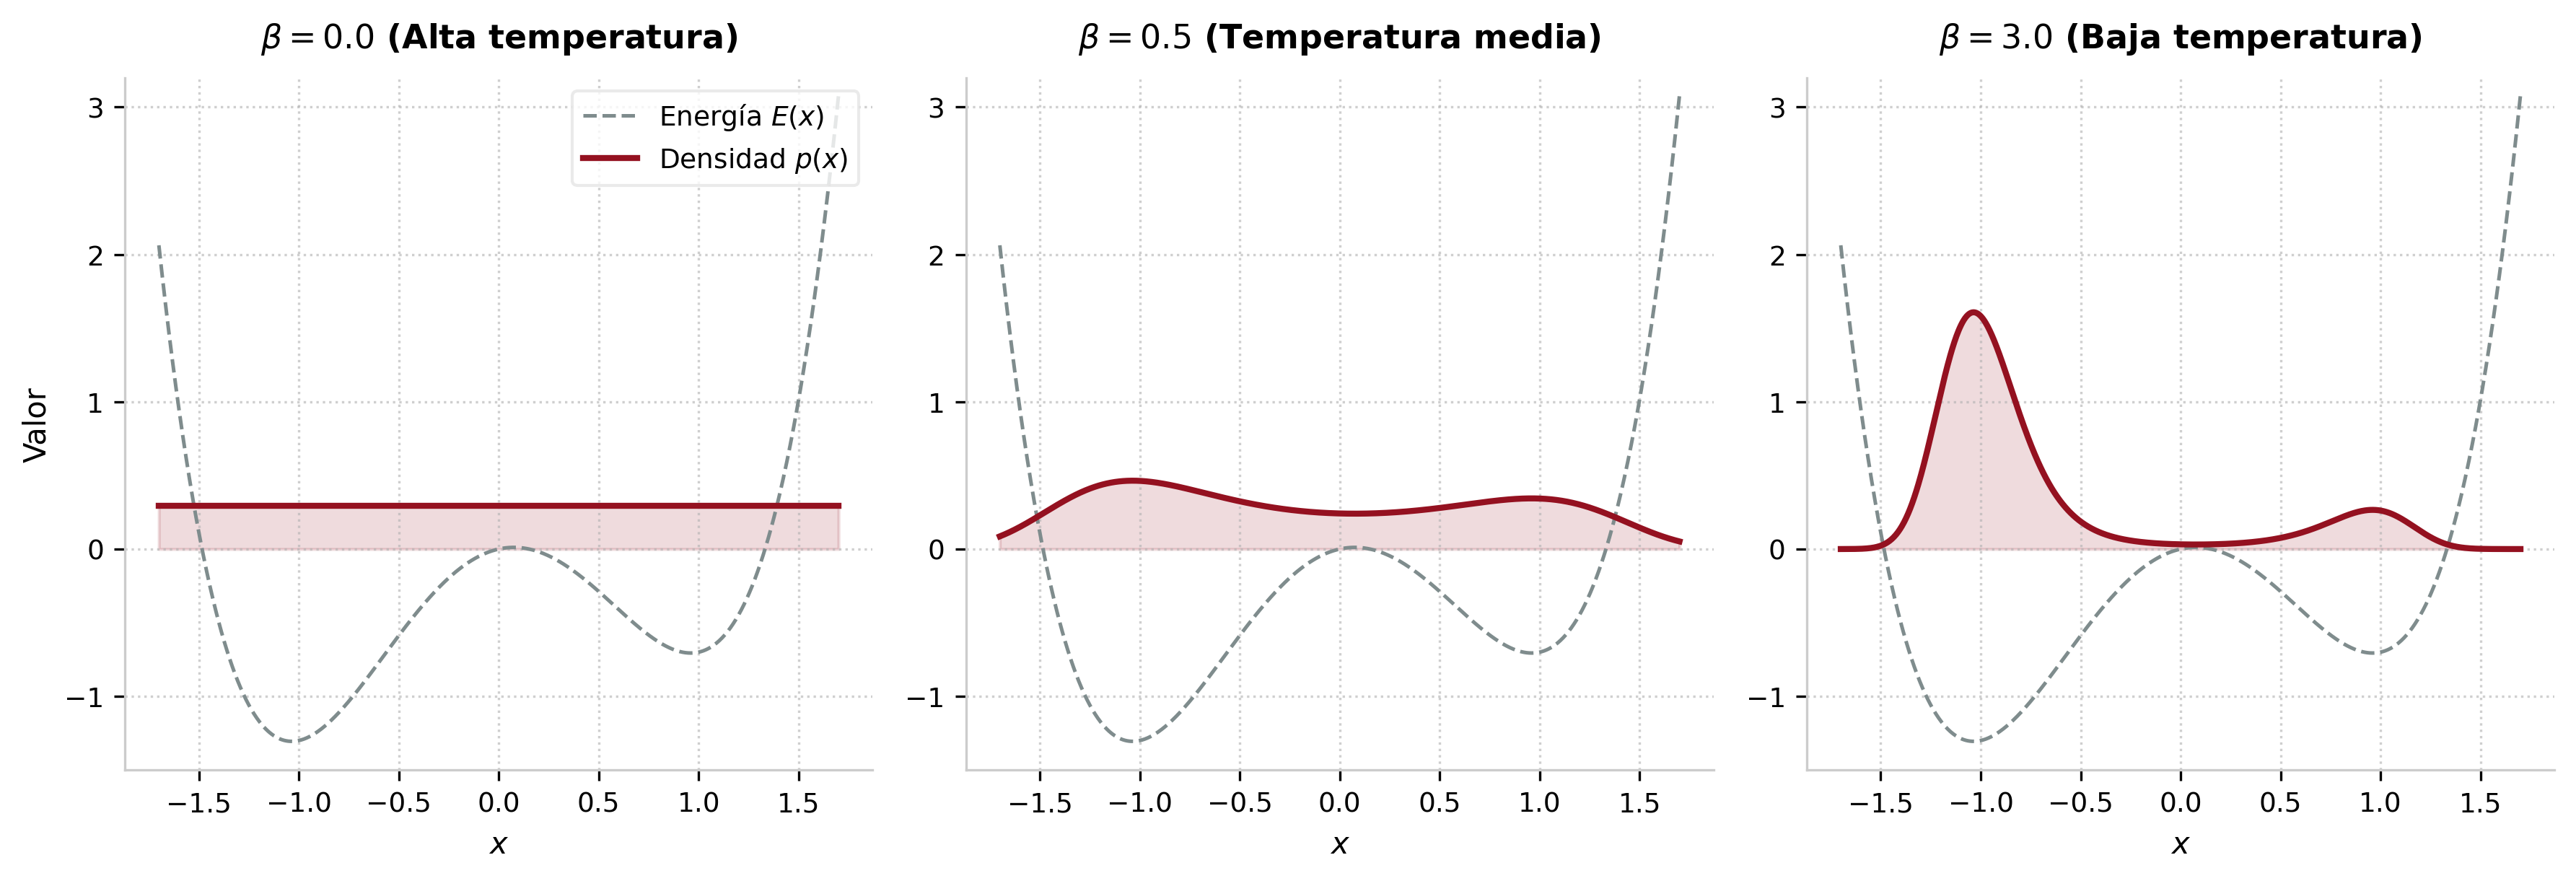
\includegraphics[width=0.95\textwidth]{beta_temperature.png}
    \caption{Evolución de la densidad de Boltzmann-Gibbs asociada a la función de energía de ejemplo $E(x) = x^4 - 2x^2 + 0.3x$, con distintos valores de $\beta$. Izquierda: $\beta = 0.0$ (alta temperatura), distribución uniforme. Centro: $\beta = 0.5$ (temperatura media), bimodalidad suave; la masa fluye con facilidad entre los valles. Derecha: $\beta = 3.0$ (baja temperatura), la masa de probabilidad se concentra fuertemente en el mínimo global de energía.}
    \label{fig:beta_temperature}
\end{figure}

\input{cap2_jaynes}

\section{El Principio de Máxima Entropía de Jaynes}
\label{sec:principio_jaynes}

La elección de la distribución condicional de Boltzmann-Gibbs de la Ecuación \eqref{eq:boltzmann_dist} puede fundamentarse en principios de teoría de la información. Es la única distribución de probabilidad que maximiza la entropía condicional sujeta a restricciones de primer momento sobre la energía.

El \textbf{Principio de Máxima Entropía de Jaynes} \cite{jaynes1957information} establece que, para una entrada fija $x \in \mathcal{X}$, la distribución de probabilidad condicional $p(y \mid x)$ que mejor representa nuestro estado de conocimiento sobre la variable de destino $y$ es aquella que \textbf{maximiza la entropía condicional de Shannon}:
\begin{equation}
\max_{p(\cdot \mid x)} \; H(p(y \mid x)) = -\sum_{y \in \mathcal{Y}} p(y \mid x) \log p(y \mid x)
\end{equation}
sujeta a las restricciones físicas impuestas por las observaciones:
\begin{align}
\text{Normalización:} \quad &\sum_{y \in \mathcal{Y}} p(y \mid x) = 1 \\
\text{Momentos de la energía:} \quad &\sum_{y \in \mathcal{Y}} p(y \mid x) f_k(x, y) = \mu_k(x), \quad \forall k=1, \dots, K
\end{align}
donde $f_k(x, y)$ son funciones de características y $\mu_k(x)$ son sus valores esperados conocidos.

La resolución analítica de este problema de optimización mediante multiplicadores de Lagrange condicionales $\lambda_k(x)$ determina de manera única que la distribución condicional de máxima entropía es:
\begin{equation}
\label{eq:solucion_jaynes}
p(y \mid x) = \frac{1}{Z(x)} \exp\left( - \sum_{k=1}^K \lambda_k(x) f_k(x, y) \right)
\end{equation}
con la función de partición $Z(x) = \sum_{y' \in \mathcal{Y}} \exp\left( - \sum_{k=1}^K \lambda_k(x) f_k(x, y') \right)$. Esta forma coincide con la distribución condicional de Boltzmann-Gibbs, donde los multiplicadores $\lambda_k(x)$ hacen el papel de la temperatura condicional inversa $\beta$.

\subsection{Conexión Adaptativa con Redes Neuronales Profundas}
\label{subsec:conexion_dnn}

La formulación de Jaynes utiliza una combinación lineal de características físicas $f_k(x, y)$ elegidas a priori:
\begin{equation}
E_{\text{Jaynes}}(x, y) = \sum_{k=1}^K \lambda_k(x) f_k(x, y)
\end{equation}
En el aprendizaje de representaciones (Representation Learning), definir manualmente estas características conjuntas para datos complejos es impracticable. Por el contrario, las Redes Neuronales Profundas resuelven esta limitación sustituyendo las funciones fijas $f_k(x, y)$ por representaciones adaptativas aprendidas de los datos.

Como se detalla en el Apéndice \ref{ap:fundamentos_dl}, una red neuronal profunda procesa la entrada conjunta $(x, y)$ a través de sus capas ocultas no lineales para calcular la energía. La salida escalar del funcional de energía $E_\theta(x, y)$ se puede interpretar en su capa de salida como una combinación lineal de las características de la última capa oculta, $\phi_k(x, y; \theta_{\text{feat}})$, ponderadas por unos pesos $w_k$ y un sesgo $b$:
\begin{equation}
E_\theta(x, y) = \sum_{k=1}^d w_k \phi_k(x, y; \theta_{\text{feat}}) + b
\end{equation}
donde $\theta = (\theta_{\text{feat}}, w, b)$ representa todos los parámetros de la red. La red neuronal no solo optimiza los multiplicadores $\lambda_k(x) = w_k$, sino que aprende de forma adaptativa las propias características $f_k(x, y)= \phi_k(x, y)$ mediante retropropagación. 

\subsection{El Dilema Probabilístico y el Salto a la Geometría}
La formulación termodinámica de Jaynes proporciona la distribución de probabilidad ideal que representa nuestro conocimiento (Máxima Entropía condicional). Sin embargo, como se detalla en la siguiente sección, el \textbf{cuello de botella computacional} de la integral de partición en espacios continuos de alta dimensión obliga a abandonar este tipo de "perfección termodinámica". 

Al prescindir de la normalización $Z$ y del "envoltorio probabilístico" $p_\theta(y \mid x)$, el modelo queda a merced de una superficie de energía \textit{no acotada probabilísticamente}. La energía pasa a interpretarse de forma puramente geométrica, computando la red, directamente un valor $E_\theta(x, y)$. Este abandono de la idea de probabilidad explica por qué en capítulos posteriores (en los que se abordan implementaciones prácticas de estos sistemas) el lenguaje de las probabilidades desaparece casi por completo en favor del álgebra lineal, la varianza y la distancia euclídea espacial.


\input{cap2_cuelloBotella}

\section{El Cuello de Botella Probabilístico: Intratabilidad de $Z(x; \theta)$}
\label{sec:cuello_botella}

Aunque la medida de Boltzmann-Gibbs condicional formaliza de manera elegante la probabilidad condicional $p_\theta(y \mid x)$ a partir de la energía $E_\theta(x, y)$, la función de partición condicional $Z(x; \theta)$ representa un cuello de botella computacional en espacios continuos de alta dimensión.

\subsection{Escenario Discreto vs. Continuo}
En espacios discretos finitos $\mathcal{Y} = \{y_1, \dots, y_K\}$ (como el vocabulario de un LLM), la función de partición se reduce a una suma finita:
\begin{equation}
Z(x; \theta) = \sum_{k=1}^K e^{-\beta E_\theta(x, y_k)}
\end{equation}
La aplicación de la normalización sobre esta suma es el operador \textbf{Softmax}, que es relativamente fácil en dominios discretos. Por el contrario, en dominios continuos como imágenes o vídeos $\mathcal{Y} \subseteq \mathbb{R}^D$, la dimensión del espacio (el número de píxeles o variables continuas) puede, fácilmente, llegar a ser del orden de $D \approx 10^6$. Es crucial distinguir esta dimensionalidad del número total de configuraciones posibles: incluso si discretizáramos cada variable en solo $256$ niveles de intensidad, la cardinalidad del espacio de búsqueda sería de $256^D \approx 10^{2.4 \times 10^6}$ combinaciones, un valor que supera por órdenes de magnitud al número de átomos del universo observable (estimado tradicionalmente en $\sim 10^{80}$). En este caso, la función de partición viene dada por la integral de Lebesgue:
\begin{equation}
Z(x; \theta) = \int_{\mathcal{Y}} e^{-\beta E_\theta(x, y')} \, dy'
\end{equation}
Esta integral carece de solución analítica para funciones de energía no lineales modeladas por redes neuronales. Además, cualquier aproximación numérica directa (como la cuadratura) es inviable debido a la maldición de la dimensionalidad (\textit{curse of dimensionality}), ya que el número de puntos de evaluación crece exponencialmente con $D$.

\subsection{El Gradiente de la Log-Partición y MCMC}
Al trabajar con funciones de verosimilitud, la intractabilidad del término de normalización $Z(x; \theta)$ se propaga al cálculo del gradiente de la log-verosimilitud. Dado que el entrenamiento de redes neuronales se basan en descenso por gradiente (Apéndice~\ref{sec:backprop}), esta intractabilidad obstaculiza este proceso de optimización. El gradiente de la función de partición logarítmica respecto a los parámetros $\theta$ se obtiene como:
\begin{align}
\nabla_\theta \log Z(x; \theta) &= \frac{1}{Z(x; \theta)} \nabla_\theta \int_{\mathcal{Y}} e^{-\beta E_\theta(x, y')} \, dy' \nonumber \\
&= -\beta \int_{\mathcal{Y}} \frac{e^{-\beta E_\theta(x, y')}}{Z(x; \theta)} \nabla_\theta E_\theta(x, y') \, dy' \nonumber \\
&= -\beta \, \mathbb{E}_{p_\theta(y \mid x)} \left[ \nabla_\theta E_\theta(x, y) \right]
\end{align}

Evaluar este gradiente exige calcular la esperanza matemática bajo la propia distribución del modelo $p_\theta(y \mid x)$. Dado que no podemos evaluar $Z(x; \theta)$, no podemos muestrear de $p_\theta$ directamente y se debe recurrir a algoritmos de Monte Carlo por Cadenas de Markov (MCMC), como las dinámicas de Langevin. En escenarios realistas de dimensiones de píxeles, MCMC es prohibitivo debido a:
\begin{itemize}
    \item \textbf{Lentitud de convergencia:} Requiere ejecutar cientos de pasos de inferencia de la red neuronal para cada muestra individual durante el bucle de optimización.
    \item \textbf{Mode Mixing:} La densidad condicional de imágenes reales es altamente multimodal. Las MCMC quedan atrapadas en mínimos locales de energía y son incapaces de transitar entre modos distantes, sesgando el gradiente del estimador.
\end{itemize}

Esta barrera  motiva el abandono del paradigma probabilístico: las JEA prescinden por completo de la normalización probabilística y de $Z(x; \theta)$, operando de forma no normalizada en el espacio latente.


\input{cap2_ebmSSL}

\section{EBMs como Marco para el Aprendizaje de Compatibilidades (SSL)}
\label{sec:ebm_ssl}

En el Aprendizaje Auto-Supervisado (SSL), el objetivo no es clasificar o predecir etiquetas, sino capturar la estructura intrínseca de los datos a partir de relaciones de consistencia. En este contexto, los EBMs se formulan sobre el espacio conjunto $\mathcal{X} \times \mathcal{Y}$ para evaluar la compatibilidad mutua de variables mediante la función de energía $E_\theta(x, y)$. Un valor de energía bajo $E_\theta(x, y)$ indica que el par de variables es consistente o compatible, mientras que un valor alto representa incompatibilidad. Este marco de compatibilidad se adapta de forma natural a las \textit{pretext tasks} (tareas auxiliares diseñadas para extraer información de supervisión de los propios datos) de SSL.

\begin{enumerate}
    \item \textbf{Predicción de regiones ocultas (Inpainting):} Sea $x_o \in \mathcal{X}_o$ la porción observada de una imagen y $x_h \in \mathcal{X}_h$ la región oculta a predecir. El EBM aprende una función de energía $E_\theta(x_o, x_h)$ que toma valores mínimos únicamente cuando la porción $x_h$ es una continuación visualmente coherente de $x_o$.
    
    \begin{figure}[htbp]
        \centering
        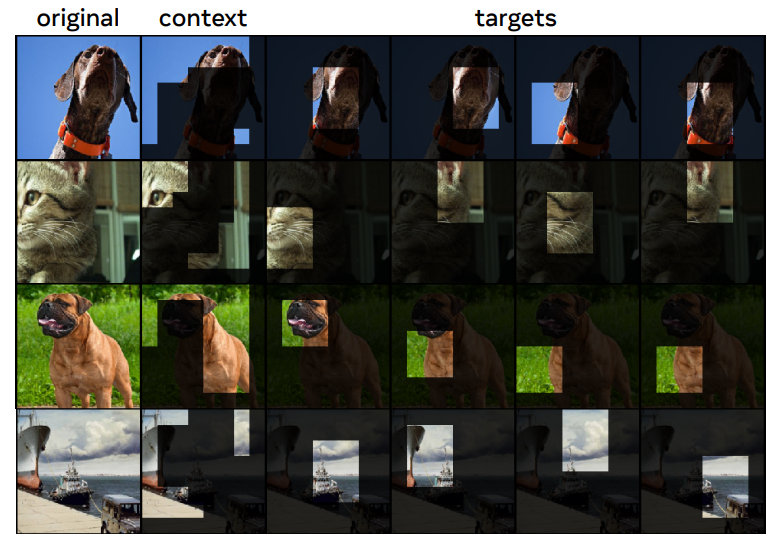
\includegraphics[width=0.8\textwidth]{SSL_inpainting.png}
        \caption{Representación de la predicción de regiones ocultas. La porción observada $x_o$ (contexto) y la porción real oculta $x_h$ (target) forman un par de baja energía $E_\theta(x_o, x_h)$, mientras que parches incorrectos elevan la energía.}
        \label{fig:ssl_inpainting}
    \end{figure}
    
    \item \textbf{Consistencia entre vistas aumentadas:} Dadas dos transformaciones aumentadas de una misma muestra $x$, denotadas como $x_1 = T_1(x)$ y $x_2 = T_2(x)$, el modelo evalúa su compatibilidad mediante $E_\theta(x_1, x_2)$. El EBM se optimiza para asignar energías bajas a las vistas que proceden de la misma muestra de origen y energías altas a vistas procedentes de muestras distintas.
\end{enumerate}

\subsection{Modelado de Compatibilidad sin Densidades de Probabilidad}
El éxito de los EBMs en SSL reside en que modelan la compatibilidad de forma directa mediante la función de energía no normalizada $E_\theta(x, y)$, evitando estimar densidades condicionales normalizadas $p_\theta(y \mid x)$. Al prescindir de la normalización, se esquiva por completo la intratabilidad del cálculo de la función de partición condicional $Z(x; \theta)$ en espacios de alta dimensión continuo como los píxeles (Sección \ref{sec:cuello_botella}).

\subsection{Las JEA como EBMs No Probabilísticos}
\label{subsec:jeas_como_ebm}

El paradigma de las \textbf{Joint Embedding Architectures (JEA)} es una realización concreta de los EBMs no probabilísticos en el espacio latente. En lugar de evaluar la compatibilidad de las entradas en el espacio físico de píxeles $\mathbb{R}^D$, las JEA proyectan $x$ e $y$ a un espacio latente de baja dimensión $\mathcal{Z} \subseteq \mathbb{R}^d$ ($d \ll D$) utilizando dos codificadores (encoders) $f_\theta$ y $g_\phi$.

Se define la \textbf{función de energía de la JEA} como la distancia euclídea al cuadrado entre los embeddings latentes de ambas variables:
\begin{equation}
\label{eq:energia_jea_latente}
E_{\theta, \phi}(x, y) = \mathcal{L}_{\text{JEA}}(x, y) = \| f_\theta(x) - g_\phi(y) \|_2^2
\end{equation}

Esta formulación aporta tres ventajas cruciales:
\begin{enumerate}
    \item \textbf{Se evita la reconstrucción:} La compatibilidad es medida directamente en $\mathcal{Z}$. Los encoders actúan como filtros de información que descartan el ruido estocástico de alta frecuencia (como detalles de fondo) y retiene únicamente características semánticas robustas.
    \item \textbf{Ausencia de normalización:} La ecuación \eqref{eq:energia_jea_latente} es estrictamente no normalizada. Evita computar la función de partición condicional $Z(x; \theta)$ sobre imágenes continuas, solucionando el cuello de botella predictivo de la integral de Lebesgue en $\mathbb{R}^D$.
    \item \textbf{Geometrización semántica:} La superficie de energía se define por la métrica de $\mathcal{Z}$. Minimizar la energía acerca las representaciones latentes de muestras coherentes, estructurando la geometría del espacio de embeddings.
\end{enumerate}

Como se detalla en el Capítulo~\ref{cap:siamesas_colapso}, la gran limitación de este enfoque no probabilístico es que, al carecer de normalización condicional o muestras negativas, el sistema tiende de forma natural al \textbf{colapso de representación}: una solución degenerada donde los encoders se vuelven constantes ($f_\theta(x) = g_\phi(y) = c$), minimizando la energía a cero de forma trivial sin extraer ninguna información semántica de la realidad.